\begin{frame}[fragile]{Forward Proxy (encaminhamento)}
    \begin{itemize}%[<+->]
        \item Atua entre o cliente e a internet É usado para controle de acesso, filtragem de conteúdo, anonimato e cache.\newline
        
        \begin{figure}
            \centering
            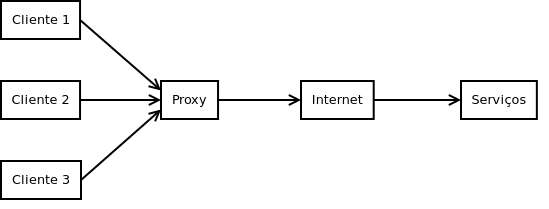
\includegraphics[width=0.7\linewidth]{contents//img/1.png}
            \caption{Forward proxy}
            \label{fig:enter-label}
        \end{figure}

    \end{itemize}
\end{frame}

\begin{frame}[fragile]{Proxy reverso}
    \begin{itemize}%[<+->]
        \item Um proxy reverso é um servidor que recebe as requisições dos clientes e as redireciona para os servidores de backend apropriados. \newline
        
        \begin{figure}
            \centering
            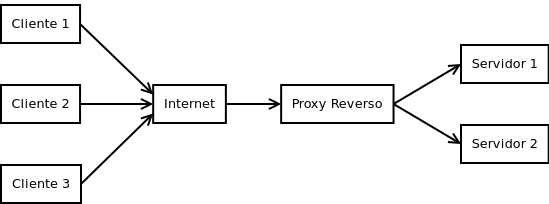
\includegraphics[width=0.7\linewidth]{contents//img/2.png}
            \caption{Proxy reverso}
            \label{fig:enter-label}
        \end{figure}
    \end{itemize}
\end{frame}